\section{Creating lightweight FAIR Digital Objects with RO-Crate}

RO-Crate {[}\href{https://doi.org/10.3233/DS-210053}{Soiland-Reyes
2022}{]} (section \ref{packaging-research-artefacts-with-ro-crate}) is a lightweight method to package research outputs along with
their metadata, based on Linked Data principles
{[}\href{https://doi.org/10.4018/jswis.2009081901}{Bizer 2009}{]} and
W3C standards. RO-Crate provides a flexible mechanism for researchers
archiving and publishing rich data packages (or any other research
outcome) by capturing their dependencies and context.

However, additional measures should be taken to ensure that a crate is
also following the FAIR principles
{[}\href{https://doi.org/10.1038/sdata.2016.18}{Wilkinson 2016}{]},
including consistent use of persistent identifiers, provenance,
community standards, clear machine/human-readable licensing for metadata
and data, and Web publication of RO-Crates.

The FAIR Digital Object (FDO) approach
{[}\href{https://doi.org/10.3390/publications8020021}{De Smedt 2020}{]}
gives a set of recommendations that aims to improve findability,
accessibility, interoperability and reproducibility for any digital
object, allowing implementation through different protocols or
standards.

Here we present how we have followed the FDO recommendations and turned
research outcomes into FDOs by publishing RO-Crates on the Web using
HTTP, following best practices for Linked Data. We highlight challenges
and advantages of the FDO approach, and reflect on what is required for
an FDO profile to achieve FAIR RO-Crates.

The implementation allows for a broad range of use cases, across
scientific domains. A minimal RO-Crate may be represented as a
persistent URI resolving to a summary website describing the outputs in
a scientific investigation
(e.g.~\url{https://w3id.org/dgarijo/ro/sepln2022} with links to the used
datasets along with software).

One of the advantages of RO-Crates is flexibility, particularly
regarding the metadata accompanying the actual research outcome.
RO-Crate extends \href{https://schema.org/}{schema.org}, a popular
vocabulary for describing resources on the Web
{[}\href{https://doi.org/10.1145/2844544}{Guha 2016}{]}. A generic
RO-Crate is not required to be typed beyond \texttt{Dataset}\footnote{To
  execute the wrapped tool, a containerized workflow engine would need
  \emph{nested containers} which are not generally recommended for
  security reasons. It is possible to work around this limitation using
  \href{https://sylabs.io/singularity/}{Singularity} or
  \href{https://docs.bioexcel.eu/cwl-best-practice-guide/devpractice/containers/conda.html}{Conda}.}
In practice, RO-Crates declare conformance to particular
\href{https://www.researchobject.org/ro-crate/profiles.html}{profiles},
allowing processing based on the specific needs and assumptions of a
community or usage scenario. This, effectively, makes RO-Crates typed
and thus machine-actionable. RO-Crate profiles serve as metadata
templates, making it easier for communities to agree and build upon
their own metadata needs.

RO-Crates have been combined with \emph{machine-actionable Data
Management Plans} (maDMPs) to automate and facilitate management of
research data {[}\href{https://doi.org/10.4126/frl01-006423291}{Miksa
2020}{]}. This mapping allows RO-Crates to be generated out of maDMPs
and vice versa. The ELIXIR Software Management Plans
{[}\href{https://doi.org/10.37044/osf.io/k8znb}{Alves 2021}{]} is
planning to move their questionnaire to a machine-actionable format with
RO-Crate. ELIXIR \href{https://biohackathon-europe.org/}{Biohackathon}
2022 will
\href{https://github.com/elixir-europe/biohackathon-projects-2022/tree/main/10}{explore}
integration of RO-Crate and the \href{https://ds-wizard.org/}{Data
Stewardship Wizard} {[}\href{https://doi.org/10.5334/dsj-2019-059}{Pergl
2019}{]} with Galaxy, which can automate FDO creation that also follows
data management plans.

A tailored RO-Crate profile has been defined to represent Electronic Lab
Notebooks (ELN) protocols bundled together with metadata and related
datasets. {[}\href{https://doi.org/10.1186/s13326-021-00257-x}{Schröder
2022}{]} uses RO-Crates to encode provenance information at different
levels, including researchers, manufacturers, biological and chemical
resources, activities, measurements, and resulting research data. The
use of RO-Crates makes it easier to programmatically question-answer
information related to the protocols, for instance activities, resources
and equipment used to create data.

Another example is \href{https://workflowhub.eu/}{WorkflowHub}
{[}\href{https://doi.org/10.5281/zenodo.4605654}{Goble 2021}{]} which
defines the
\href{https://w3id.org/workflowhub/workflow-ro-crate/1.0}{Workflow
RO-Crate} profile
{[}\href{https://w3id.org/workflowhub/workflow-ro-crate/1.0}{Bacall
2022}{]}, imposing additional constraints such as the presence of a main
workflow and a license. It also specifies which entity types and
properties must be used to provide such information, implicitly defining
a set of operations (e.g., get the main workflow and its language) that
are valid on all complying crates. The workflow system Galaxy
{[}\href{https://doi.org/10.1093/nar/gkac247}{Galaxy 2022}{]} retrieves
such Workflow Crates using
\href{https://about.workflowhub.eu/developer/trs/}{GA4GH TRS API}.

The workflow profile has been further extended (with OOP-like
inheritance) in
\href{https://crs4.github.io/life_monitor/workflow_testing_ro_crate}{Workflow
Testing RO-Crate}, adding formal workflow testing components: this adds
operations such as getting remote test instances and test definitions,
used by the \href{https://www.lifemonitor.eu/}{LifeMonitor} service to
keep track of the health status of multiple published workflows.

While RO-Crates use Web technologies, they are also
\emph{self-contained}, moving data along with their metadata. This is a
powerful construct for interoperability across FAIR repositories, but
this raises some challenges with regards to mutability and persistence
of crates.

To illustrate how such challenges can be handled, we detail how the
WorkflowHub repository follows several FDO principles:

\begin{enumerate}
\def\labelenumi{\arabic{enumi}.}
\tightlist
\item
  Workflow entries must be \emph{frozen} for editing and have complete
  kernel metadata (title, authors, license, description) {[}FDOF4{]}
  before they can be assigned a persistent identifier,
  e.g.~\url{https://doi.org/10.48546/workflowhub.workflow.255.1}
  {[}FDOF1{]}
\item
  Computational workflows can be composed of multiple files used as a
  whole, e.g.~CWL files in a GitHub repository. These are snapshotted as
  a single RO-Crate ZIP, indicating the main workflow. {[}FDF11{]}
\item
  PID resolution can content-negotiate to Datacite's PID metadata
  {[}FDOF2{]} or use \href{https://signposting.org/FAIR/}{FAIR
  Signposting} to find an RO-Crate containing the workflow {[}FDOF3{]}
  and richer JSON-LD metadata resources {[}FDOF5,FDOF8{]}, see
  \protect\hyperlink{fig:signposting}{Figure 1}
\item
  Metadata uses schema.org {[}FDOF7{]} following the community-developed
  Bioschemas
  \href{https://bioschemas.org/profiles/ComputationalWorkflow/1.0-RELEASE}{ComputationalWorkflow}
  profile {[}FDOF10{]}.
\item
  Workflows are discovered using
  the\href{https://about.workflowhub.eu/developer/trs/}{GA4GH TRS API}
  {[}FDOF5,FDOF6,FDOF11{]} and created/modified using
  \href{https://workflowhub.eu/api}{CRUD operations} {[}FDOF6{]}
\item
  The RO-Crate profile, effectively the FDO Type {[}FDOF7{]}, is
  declared as \url{https://w3id.org/workflowhub/workflow-ro-crate/1.0};
  the workflow language
  (e.g.~\url{https://w3id.org/workflowhub/workflow-ro-crate\#galaxy} is
  defined in metadata of the main workflow.
\end{enumerate}

\begin{figure}
  \centering
%      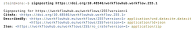
\includegraphics[width=0.3\textwidth]{signposting.svg}
  \caption{FAIR Signposting.}
  \label{fig:signposting}
\end{figure} 


\{\{\textless{} figure src=``signposting.svg'' id=``fig:signposting''
width=``100\%'' title=``FAIR Signposting''
caption=``\href{https://signposting.org/FAIR/}{FAIR Signposting} on a
workflow PID
{[}\href{https://doi.org/10.48546/workflowhub.workflow.255.1}{Bayarri
2022}{]} discovered from HTTP \texttt{Link:} headers using the
\href{https://pypi.org/project/signposting/}{Signposting tool} shows
machine-actionable navigation to content-negotiate for the metadata
FDOs, as well as download bit sequence {[}FDOF3{]} as an RO-Crate zip.
\href{https://workflowhub.eu/workflows/255.jsonld}{JSON-LD from
workflowhub.eu} follows the BioSchemas
\href{https://bioschemas.org/profiles/ComputationalWorkflow/1.0-RELEASE}{ComputationalWorkflow
profile} to give workflow details not included in DataCite's
\href{https://data.crosscite.org/application/ld+json/10.48546/workflowhub.workflow.255.1}{general
JSON-LD}.'' \textgreater\}\}

Further work on RO-Crate profiles include to formalise links to the API
operations and repositories {[}FDOF5,FDOF7{]}, to include PIDs of
profiles and types in the FAIR Signposting, and HTTP navigation to
individual resources within the RO-Crate.

RO-Crate has shown a broad adoption by communities across many
scientific disciplines, providing a lightweight, and therefore easy to
adopt, approach to generating FAIR Digital Objects. It is rapidly
becoming an integral part of the interoperability fabric between the
different components as demonstrated here for WorkflowHub, contributing
to building the European Open Science Cloud.
